\chapter{Resultados e Discussão}
\label{cap:resultados}

Esta seção apresenta os principais resultados obtidos ao decorrer do desenvolvimento do sistema automatizado de limpeza e manutenção de piscinas, analisando seu desempenho operacional e os desafios técnicos enfrentados. Os aspectos discutidos são a integração do protótipo físico, a usabilidade da interface de controle desenvolvida e a validação dos dados coletados, destacando os avanços alcançados em relação aos métodos manuais tradicionais e as limitações observadas no modelo experimental.

\section{Integração do Protótipo Físico}

O desenvolvimento do protótipo possibilitou a consolidação da arquitetura proposta na fase de Elaboração. O protótipo foi acoplado em uma caixa de isopor com o intuito de simular um ambiente real e fazer um revestimento dos componentes que o integram, garantindo a proteção dos circuitos contra respingos, considerando o ambiente úmido de operação. A disposição dos sensores de pH, turbidez, temperatura e nível no reservatório de teste demonstrou-se eficaz para a leitura contínua, garantindo uma boa confiabilidade no quesito qualidade dos dados.

A Figura \ref{fig:prototipo_final} apresenta a visão geral do protótipo montado, demonstrando a conexão entre a central de controle e os dispositivos imersos.

\begin{figure}[H]
    \centering
    \caption{Protótipo final do sistema de automação montado.}
    \label{fig:prototipo_final}
    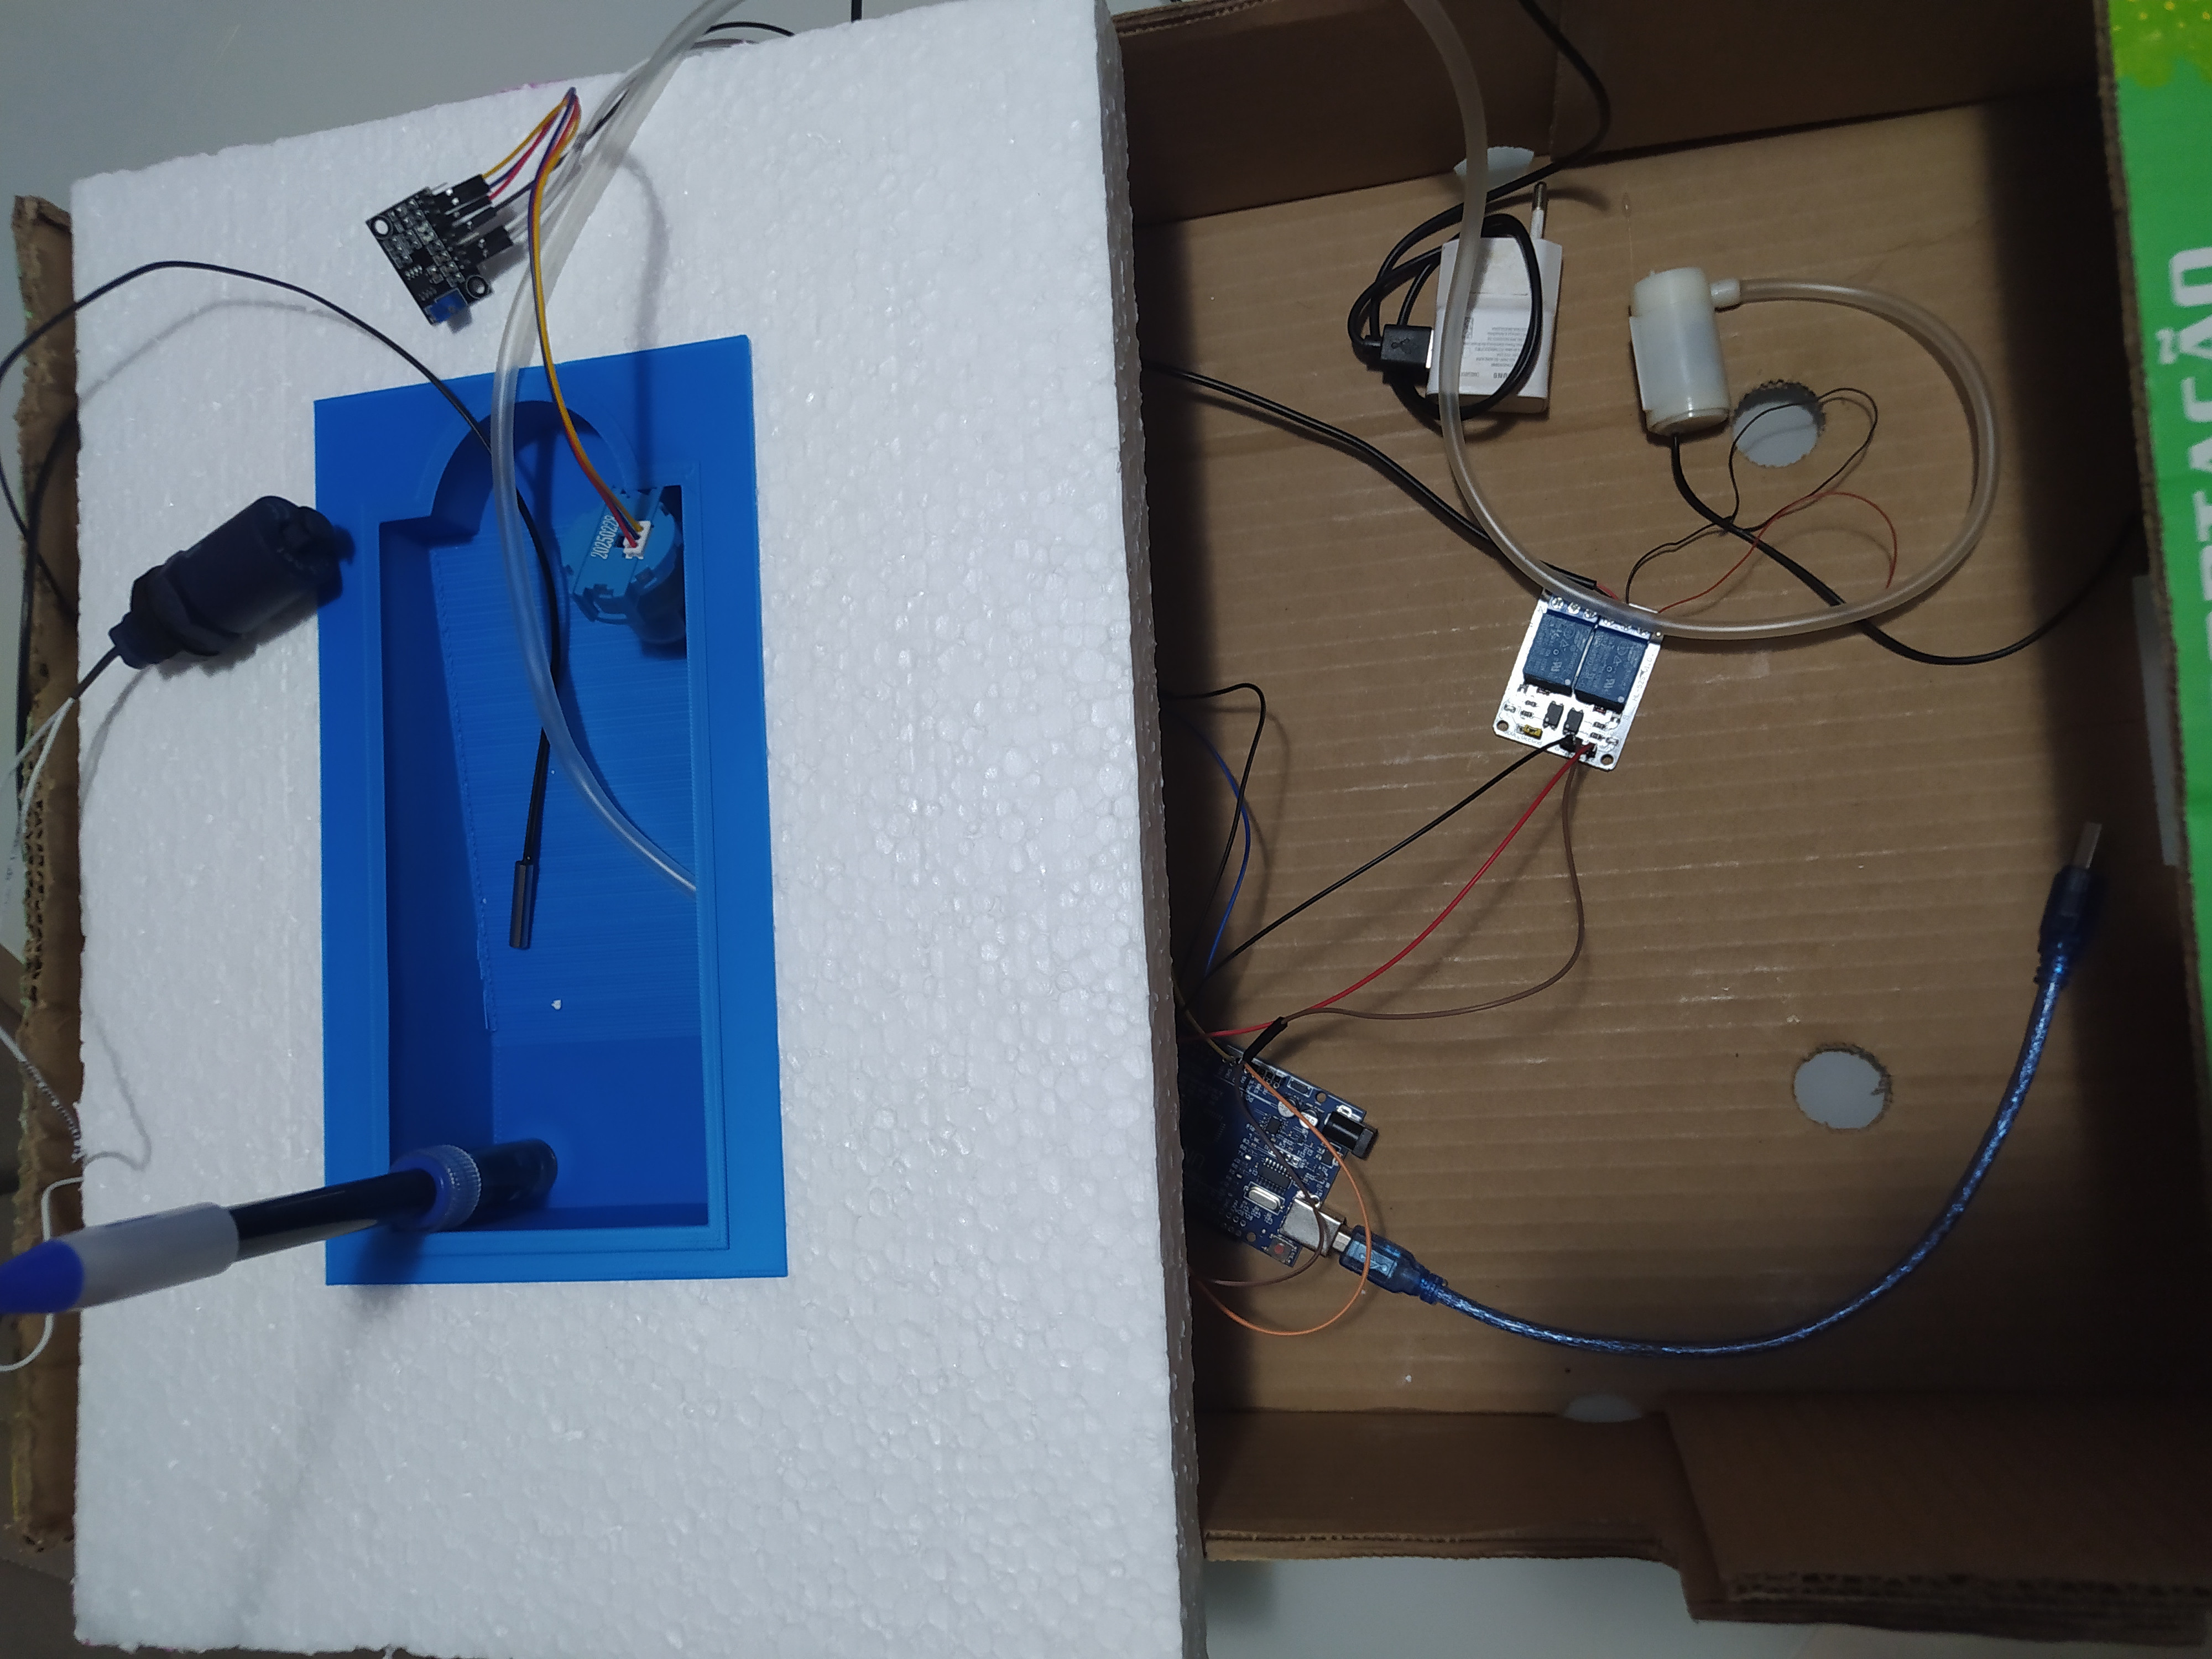
\includegraphics[width=0.8\textwidth]{imagens/prototipoFinal.png}
    \caption*{Fonte: Autoria própria (2025).}
\end{figure}

\vspace{5em}

Durante os testes de integração, o sistema de atuadores respondeu conforme o esperado, com o acionamento da bomba via relé ocorrendo sem atrasos perceptíveis. Entretanto, nas etapas iniciais de validação, foi indentificado um problema: o acionamento da bomba gerava ruídos eletromagnéticos e picos de tensão que interferiam no circuito do microcontrolador, comprometendo a estabilidade das leituras dos sensores e da própria bomba.

Tal problema foi solucionado com a substituição do módulo de acionamento simples por um módulo relé com isolamento via optoacoplador. Essa alteração garantiu o isolamento galvânico entre o circuito de potência e o circuito lógico do Arduino, eliminando as interferências indentificadas. A Figura \ref{fig:rele_opto} apresenta o componente adotado para mitigar essa falha.

\begin{figure}[H]
    \centering
    \caption{Relé com optoacoplador}
    \label{fig:rele_opto}
    \includegraphics[width=0.60\textwidth]{imagens/releFinal.jpeg}
    \caption*{Fonte: Autoria própria (2025).}
\end{figure}

Junto a isso, foram encontrados alguns problemas esperados, como o sensor de pH, que chegou descalibrado de fábrica e precisou ser calibrado no módulo ao qual foi acoplado. O ajuste foi realizado via \textit{hardware}, atuando no potenciômetro (\textit{trimpot}) de \textit{offset} da placa condicionadora para alinhar a tensão de saída ao valor de referência. A calibração foi validada utilizando uma garrafa de água mineral fechada, conforme evidenciado na Figura \ref{fig:sensorpH:sendoCalibrado}, que possui pH declarado de 6,98. Após o ajuste, o sensor obteve leituras entre 6,78 e 6,80, validando a precisão.

\begin{figure}[H]
    \centering
    \caption{Validação sensor de pH}
    \label{fig:sensorpH:sendoCalibrado}
    \includegraphics[width=1.00\textwidth]{imagens/calibracaoSensorPh.png}
    \caption*{Fonte: Autoria própria (2025).}
\end{figure}

Além disso, o sensor de temperatura também apresentou desvios de fábrica. A calibração foi realizada via código, aplicando-se um fator de correção à equação do divisor de tensão para compensar a variação na resistência nominal do termistor (NTC). A validação foi feita utilizando um termômetro de piscina como referência, comparando a leitura da temperatura da água (medindo 25.7) com a leitura do sensor (25.93), o que validou o componente, como mostrado na Figura \ref{fig:sensorTemperatura:sendoCalibrado}.

\begin{figure}[H]
    \centering
    \caption{Validação sensor de temperatura}
    \label{fig:sensorTemperatura:sendoCalibrado}
    \includegraphics[width=1.00\textwidth]{imagens/calibrandoSesorTemperatura.png}
    \caption*{Fonte: Autoria própria (2025).}
\end{figure}

\vspace{5em}

\section{Interface de Controle e Monitoramento}

O software desenvolvido para a interface do usuário (Front-end em React) foi projetado para centralizar as informações complexas em um \textit{dashboard} intuitivo, abstraindo a complexidade técnica dos sensores. Diferente de soluções que exigem interpretação de códigos ou acesso direto ao hardware por meio de \textit{displays LCD}, a interface apresenta os indicadores de qualidade da água de forma visual e direta.

Ao acessar o sistema, o usuário visualiza em tempo real os cards de status da piscina. A comunicação com o \textit{Back-end} (Spring Boot) garante que os dados exibidos sejam atualizados periodicamente, permitindo acompanhar a evolução do tratamento. Além do monitoramento passivo, a interface oferece controles ativos, permitindo ligar ou desligar a filtragem manualmente, sobrepondo a automação em casos de necessidade de manutenção específica.

A Figura \ref{fig:dashboard_web} ilustra a tela principal do sistema, onde são exibidos os valores atuais de pH, temperatura, turbidez e o estado da bomba.

\begin{figure}[H]
    \centering
    \caption{Interface Web: Dashboard de monitoramento em tempo real.}
    \label{fig:dashboard_web}
    \includegraphics[width=1.0\textwidth]{imagens/printSistema.png}
    \caption*{Fonte: Autoria própria (2025).}
\end{figure}

\vspace{5em}

\section{Análise de Desempenho e Discussão}

Os testes práticos realizados no cenário de validação demonstraram que o sistema é capaz de realizar o ciclo completo de automação: leitura, processamento, envio e atuação.

No que tange à precisão das leituras, o sensor de temperatura NTC 10K apresentou alta estabilidade, com variações desprezíveis em relação ao termômetro de referência. Já os sensores de qualidade da água exigiram um tratamento de software e hardware mais robusto. Observou-se que, sem a aplicação de filtros de média móvel no firmware do Arduino, as leituras apresentavam oscilações momentâneas (ruído), o que poderia levar a acionamentos indevidos da bomba. Com a implementação da filtragem digital, o sistema atingiu uma estabilidade satisfatória para uso doméstico.

A latência da comunicação, um dos requisitos não funcionais críticos, manteve-se dentro do aceitável para aplicações IoT residenciais. O tempo médio entre a mudança de estado físico (ex: sensor de nível detectando falta d'água) e a atualização na interface web foi inferior a 5 segundos na maioria dos testes, validando a eficiência da arquitetura distribuída baseada em API REST.

As limitações encontradas, principalmente relacionadas à sensibilidade dos sensores analógicos de baixo custo e à dependência da estabilidade da rede Wi-Fi local, apontam caminhos para evoluções futuras do projeto, as quais serão detalhadas nas considerações finais.

\section{Trabalhos futuros}

    Integrar um sensor de cloro livre (ORP), completando o ciclo de automação química, bem como implementar algoritmos de aprendizado de máquina voltados para manutenção preditiva, com o objetivo de antecipar falhas em bombas e sensores com base no histórico operacional. Implementar o sistema em até duas piscinas de alvenaria em escala real, proporcionando uma melhor visualização da capacidade total do sistema e permitindo sua expansão. Aumento na escalabilidade do sistema possibilitando a adição de mais piscinas e usuários, ampliando sua aplicabilidade. Por fim, a adição de uma arquitetura orienta a eventos, utilizado o padrão de projeto Observer no \textit{back-end}. Essa abordagem permitirá que a interface web possa ser comunicada possivamente e de forma instantanea assim que novas leituras forem sendo processadas, eliminando a nescessidade de requisições cíclicas (\textit{polling})\footnote{É uma técnica onde um programa verifica repetidamente o status de um dispositivo externo ou de um servidor em intervalos regulares para saber se há novos dados ou eventos}, otimizando todo o processo de coleta e processamento.

    